\subsection{Figure}

In figure \ref{fig:life_expectancy} we can see the relationship between life expectancy and GDP per capita. The data shows a positive correlation, indicating that as GDP per capita increases, life expectancy tends to increase as well. This is consistent with the hypothesis that higher income levels lead to better health outcomes.
However, it is important to note that this relationship may not be causal, as other factors such as healthcare access, education, and social determinants of health also play a significant role in life expectancy.
In addition, the relationship is not linear, as there are diminishing returns to life expectancy at higher levels of GDP per capita. This suggests that while economic growth can improve health outcomes, there are limits to how much it can do so.

\begin{figure}[htbp]
\centering
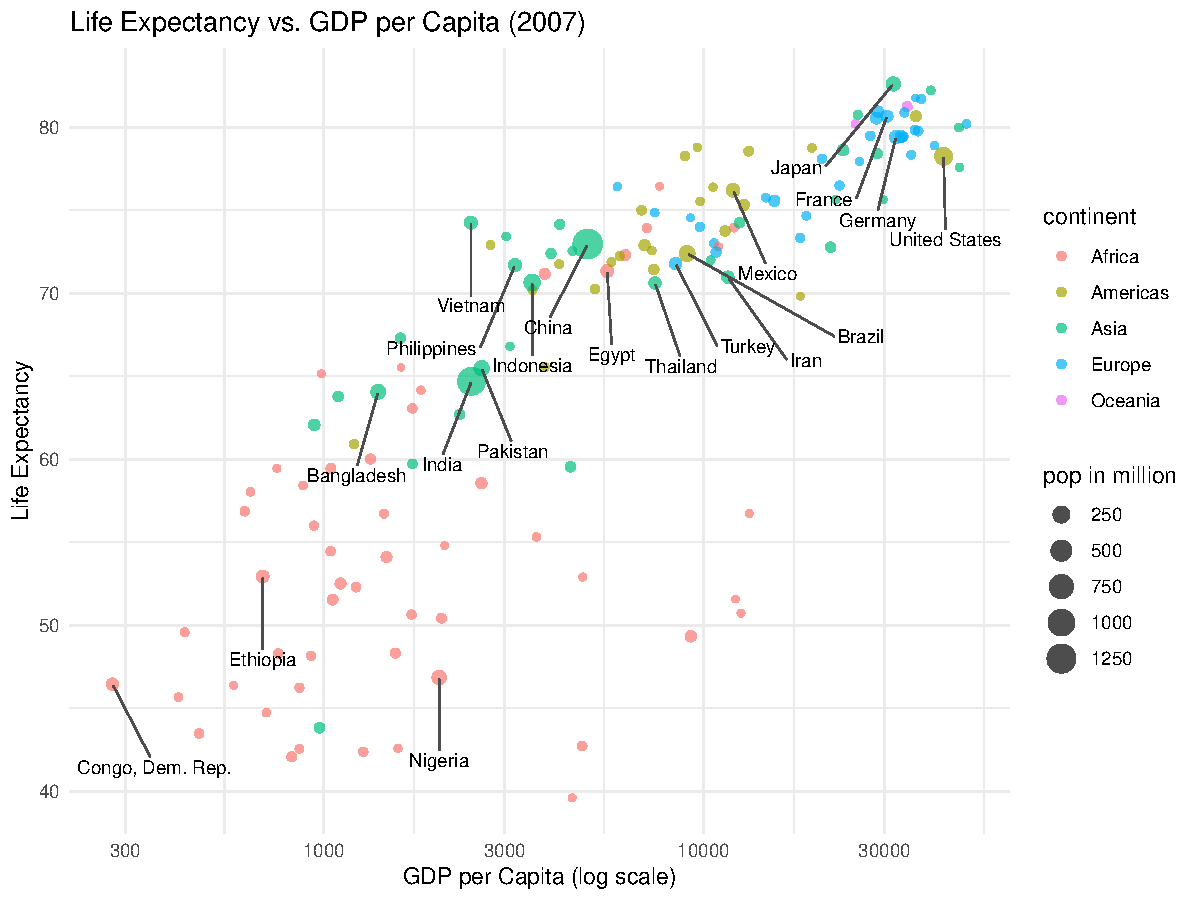
\includegraphics[width=0.9\textwidth]{../../output/figures/fig_life_expectancy.pdf}
\caption{Life Expectancy vs. GDP per Capita}
\label{fig:life_expectancy}
\end{figure}


\textcolor{gray}{\lipsum[6-8]}

\subsection{Table}

See table \ref{tab:summary-table} for a summary of the results.

\begin{table}[!t]
\caption{Summary Statistics by Continent (2007) \label{tab:summary-table}} 
\fontsize{12.0pt}{14.4pt}\selectfont
\begin{tabular*}{\linewidth}{@{\extracolsep{\fill}}crr}
\toprule
continent & mean\_lifeExp & mean\_gdpPercap \\ 
\midrule\addlinespace[2.5pt]
Africa & 54.8 & 3089.0 \\ 
Americas & 73.6 & 11003.0 \\ 
Asia & 70.7 & 12473.0 \\ 
Europe & 77.6 & 25054.5 \\ 
Oceania & 80.7 & 29810.2 \\ 
\bottomrule
\end{tabular*}
\end{table}



\textcolor{gray}{\lipsum[9-10]}